%-----------------------------------------------------------------------
%                                                                 aa.tex
% AA vers. 9.3, LaTeX class for Astronomy & Astrophysics
% Demonstration file
%                                                       (c) EDP Sciences
%-----------------------------------------------------------------------
%
%\documentclass[referee]{aa}    % for a referee version
%\documentclass[onecolumn]{aa}  % for a paper on 1 column  
%\documentclass[longauth]{aa}   % for long lists of authors and/or affiliations. 
                                % This command displays the first eight authors on page 1
                                % and shift the whole list after the references.
                                % Ensure to separate each author with the \and command (see below)
%\documentclass[letter]{aa}     % for the letters
%\documentclass[bibyear]{aa}    % if the references are not structured
                                % according to the author-year natbib style

\documentclass{aa}  

\usepackage{graphicx}
\usepackage{txfonts}
\usepackage{lipsum}
\usepackage{subcaption}         % necessary for continued figures, example in section 3
                                % and appendix
\usepackage{lscape}             % to rotate a single page table, example in appendix.
                                % For landscape tables, see the longtable examples.
\usepackage{placeins}           % useful with \FloatBarrier, to keep 
                                % onecolumn floats from drifting to the next section
                                
%%%%%%%%%%%%%%%%%%%%%%%%%%%%%%%%%%%%%%%%
\usepackage[]{hyperref}
\hypersetup{
    colorlinks=true,
    linkcolor=blue,
    filecolor=magenta,
    urlcolor=blue,
    citecolor=blue,
}


% extra commands
\newcommand{\V}{{\rm v}}
\newcommand{\vmax}{\V_{\rm max}}
\newcommand{\vcirc}{\V_{\rm circ}}
\newcommand{\rmax}{r_{\rm max}}
\newcommand{\kpc}{{\rm kpc}}
\newcommand{\Gyr}{{\rm Gyr}}
\newcommand{\kms}{{\rm km\,s^{-1}}}
\newcommand{\masyr}{{\rm mas\,yr^{-1}}}
\newcommand{\Mo}{M_\odot}

\newcommand{\agama}{{\tt Agama}}
\newcommand{\gadget}{{\tt Gadget-4}}
\newcommand{\smallperi}{{\tt smallperi}}
\newcommand{\LCDM}{$\Lambda$CDM}


%%% citepos command
\makeatletter
\DeclareRobustCommand\citepos
  {\begingroup
   \let\NAT@nmfmt\NAT@posfmt% ...except with a different name format
   \NAT@swafalse\let\NAT@ctype\z@\NAT@partrue
   \@ifstar{\NAT@fulltrue\NAT@citetp}{\NAT@fullfalse\NAT@citetp}}

\let\NAT@orig@nmfmt\NAT@nmfmt
\def\NAT@posfmt#1{\NAT@orig@nmfmt{#1's}}

\makeatother




\begin{document}

%%%%%%%%%%%%%%%%%%%%%%%%%%%%%%%%%%%%%%%%
% if you use custom commands in your title,
% ensure to check your title when submitting!
%%%%%%%%%%%%%%%%%%%%%%%%%%%%%%%%%%%%%%%%
\title{Could tides explain the extended stellar densities of the Sculptor and Ursa Minor dwarfs?}

%%%%%%%%%%%%%%%%%%%%%%%%%%%%%%%%%%%%%%%% % Please separate each author with the \and command
%
% Please do not include ORCIDs next to author names.
% Only ORCIDs authenticated by individual authors in EDPS
% editorial system will be taken into account.
% ORCIDs included here will be removed.
%%%%%%%%%%%%%%%%%%%%%%%%%%%%%%%%%%%%%%%%

   \author{D. A. Boyea\inst{1}
        \and others
        }

        \institute{%
            Department of Physics \& Astronomy, University of Victoria, Finnerty Road, Victoria, British Columbia V8A 1A1, Canada
             \email{danielaboyea@gmail.com}
             %\thanks{Shows the usage of elements in the institute field}
            \and others\\ }

   \date{Received December XX, 20XX}

% \abstract{}{}{}{}{}
% 5 {} token are mandatory
 
  \abstract
  % context heading (optional)
   {Most dwarf spheroidals (dSph) of the Milky Way have light profiles following an exponential law, with a sharply declining outer density. However, Sculptor (Scl) and Ursa Minor (UMi) dSphs show an excess of stars at large radii.}
  % aims heading (mandatory)
   {We investigate whether tides may produce these extended light profiles.}
  % methods heading (mandatory)
   {We conduct idealized N-body simulations of both galaxies in the tidal field of the Milky Way and Large Magellanic Cloud (LMC). }
  % results heading (mandatory)
   {Tides affect neither galaxy strongly. Because the LMC perturbs Scl's orbit, Scl has few pericentres and the stellar component evolves little. UMi instead loses about 95\% of its dark matter mass, but the stars would still appear unaffected with current observations. }
  % conclusions heading (optional), leave it empty if necessary
   {The outer stellar excess in Scl and UMi are likely not of tidal origin. Instead, these features are likely innate, possibly explained by past mergers, accretion, or star formation episodes. }

   \keywords{Galaxies: dwarf --
       Galaxies: kinematics and dynamics --
       Local Group
               }

   \maketitle


%%%%%%%%%%%%%%%%%%%%%%%%%%%%%%%%%%%%%%%%%%%%%%%%%%%%%%%%%%%%%%
\section{Introduction}

Since \citet{faber+lin1983}, exponential surface density profiles have been commonly used to describe dwarf spheroidal (dSph) galaxies \citep[e.g.,][]{binggeli+sandage+tarenghi1984, mateo1998, mcconnachie+irwin2006, cicuendez+2018, kowalczyk+2013, martin+2016, MV2020a, battaglia+2022}.
However, the Sculptor (Scl) and Ursa Minor (UMi) dSphs show clear deviations from an exponential profile (Fig.~\ref{fig:observed_density_profiles}; e.g., \citealt{eskridge1988, IH1995, martinez-delgado+2001, walcher+2003, palma+2003}). This excess of stars at large radii was often speculated to be tidal interaction \citep[e.g.][]{innanen+papp1979, walcher+2003} or sometimes a `halo'of stars surrounding the dwarf \citep{westfall+2006}.
Most recently, \citet{sestito+2023a, sestito+2023b} report a
`kink' in the density profile of each galaxy. They spectroscopically
confirm distant members out to ${\sim}10$ half-light
radii from the centre of each dwarf. If these dwarfs had exponential
profiles, then these far-outlying stars should be much
rarer. We aim to test whether tides may form the extended stellar densities of Scl and UMi.

Cosmological simulations struggle to resolve tidal effects on dwarfs. Dwarfs are 
often near the resolution limit and vulnerable to artificial disruption
\citep[e.g.,][]{vandenbosch+2018, santos-santos+2025}. To overcome
these challenges, idealized simulations model a single subhalo in an
analytic host potential, achieving excellent numerical convergence \citep[e.g.,][]{hayashi+2003, bullock+johnston2005, klimentowski+2009, ogiya+2019}.
From these simulations, tidally stripped stars form \emph{tidal
streams}---stellar tails with a bulk velocity gradient
\citep[e.g.,][]{moore+davis1994, johnston+spergel+hernquist1995, read+2006}.
Most mass loss happens near pericentre, where tides are strongest.
However, the central structure of a dwarf galaxy often remains
undisturbed \citep{oh+lin+aarseth1995, piatek+pryor1995}. 
To first order, tidal mass loss peels away the outer layers of a dwarf
galaxy in energy space (\citealt{choi+weinberg+katz2009, drakos+taylor+benson2020, drakos+taylor+benson2022, amorisco2021}; or more generally, the adiabatic removal of stars on unbound orbits in \citealt{stucker+2023}). The most loosely bound particles are removed first---substantial dark matter mass can be removed before affecting the stellar component.

Improved orbital constraints and Milky Way
potential models have enabled precise dynamical modeling of dwarf galaxies.
Simulations tuned to Fornax \citep{battaglia+sollima+nipoti2015, borukhovetskaya+2022, dicintio+2024},
Scl \citep{iorio+2019}, or MW classicals\footnote{We define classicals to be dwarfs with absolute magnitudes between $-7.7$ and $-14$.} in general \citep{tchiorniy+genina2025} often find tides play a minor role in the stellar evolution of dwarf classicals. However, modeling tidal evolution under the Large Magellanic Cloud (LMC) has not yet been considered for most classical dSphs.

Two radii provide estimates of where tidal effects occur.
The \textbf{Jacobi radius}, $r_{\rm J}$. approximates the radius where stars
become unbound in a galaxy\footnote{ 
    While strictly valid only for circular orbits, assuming
\(r_{\rm peri}\) for the host-dwarf distance works as most stars are
lost during pericentric passages. $r_{\rm J}$ solves
}
\begin{equation}\label{eq:r_jacobi}
    3\bar \rho_{\rm MW}(r_{\rm peri}) \approx \bar \rho_{\rm dwarf}(r_J),
\end{equation}
given the mean enclosed  density of the host at pericentre $\bar \rho_{\rm MW}(r_{\rm peri})$,
and the mean enclosed satellite density $\bar \rho_{\rm dwarf}(r)$ \citep[eq. 7-84]{BT1987}.
If \(r_J\) is comparable to
the visible extent of a galaxy, we should expect to find clear signs of
tidal disturbance. 
The \textbf{break radius}, as defined in
\citet{penarrubia+2009}, marks the outermost dynamically-relaxed radius after pericentric passage. Based on the velocity dispersion, \(\sigma_v\), and time elapsed
since pericentre, \(\Delta t\), the break radius is
\begin{equation}\label{eq:r_break}
    r_{\rm break} = C\,\sigma_{v}\,\Delta t
\end{equation} 
where the empirical constant is \(C \approx 0.55\).

Building on this body of work, we will use idealized simulations to
understand the severity of tidal effects on Scl and UMi.

\section{{\it Gaia} density profiles}

Measuring the light profile of a resolved galaxy requires careful
consideration of whether any given star belongs to the system or not.
Without removing contamination from foreground/background sources, faint
features may be lost in the noise or be of uncertain association. In addition to colours and magnitudes, \emph{Gaia} now \citep{gaiacollaboration+2023} provides stellar parallax and proper motion which improve membership assignment.


Here, we use the \citepos[hereafter J+24]{jensen+2024} membership
probabilities from \emph{Gaia} data.\footnotemark{} J+24 used a Bayesian framework
incorporating proper motion, colour--magnitude diagram, and
spatial information to determine the probability that a given star
belongs to the satellite, $P_{\rm sat}$. By accounting for proper motions
in particular, J+24 produced low contamination samples of candidate
member stars out to large distances from a dwarf galaxy. J+24 extended
the algorithm presented in \citet{MV2020a, MV2020b} by additionally
including a secondary, extended spatial component, J+24 detected
candidate members out to ${\sim}10$ half-light radii from the
centres of some galaxies (\(R_h\)). Similar recent work includes
\citet{pace+li2019}; \citet{battaglia+2022}; \citet{pace+erkal+li2022};
\citet{qi+2022}.

\footnotetext{
We use
the \(P_{\rm sat}\) values from the elliptical 2-component runs if a
galaxy shows evidence for an outer component, the 1-component run
otherwise. 
}

For our sample, we adopt a minimum probability of
\(P_{\rm sat} = 0.2\).
%We do not filter on magnitudes explicitly, but J+24's quality cuts typically only include stars with \(G < 21\).
Most stars have \(P_{\rm  sat}\) values which are nearly 0 or 1, so the exact
choice of probability threshold has little effect on the resulting sample. Even
at the probability threshold of 0.2, the purity remains high when validated
against spectroscopic line-of-sight (LOS) velocities (${\sim}90\%$,
J+24).\footnotemark{} However, we find that our conclusions are unchanged when
limiting samples to only the brightest stars. Altogether, the J+24 method
provides a high-quality, low-contamination sample of dwarf galaxy candidate
member stars, which we will now investigate in further detail.

\footnotetext{This
  would indicate that the J+24 model probabilities are miss-calibrated.
  However, most LOS surveys of dwarf galaxies select brighter stars
  (which have better \emph{Gaia} measurements) and likely members,
  complicating the interpretation of this purity estimate.}


Fig.~\ref{fig:observed_density_profiles} compares the density
profiles of Scl, UMi, and eight other classical dwarf
galaxies.\footnote{
    We define classicals to be non-Magellanic dwarfs brighter than
    $Mv = -7.7$, i.e., Sagittarius, Fornax, Leo I, Sculptor, Antlia II, Leo II,
    Carina, Draco, Ursa Minor, Canes Venatici I, Sextans I, and Crater II. Of
    these dwarfs, we exclude Antlia II, due to the extremely high background,
    and Sagittarius, which was not included in J+24. 
}
All of the classical dwarfs appear to be well
described by an exponential profile in the inner regions.\footnote{
    Comparing
    density profiles of dwarf galaxies is complicated by variations in the
    effective depth between galaxies. However, the deviations between Scl,
    UMi, and other galaxies are apparent even where the data is complete
    across all dwarfs.} 
In the outer regions, however, Scl and Ursa
Minor deviate and show a clear outer excess over an exponential law
(solid black line). These galaxies are better fit by a Plummer law
(dashed black line). The deviation from an exponential grows outwards,
and at \(\sim 8 R_h\), may reach 2 orders of magnitude. 


\begin{figure}
    \centering
    \includegraphics{figures/classical_dwarf_profiles.pdf}
    \caption{
        The density profiles of
        Sculptor (orange squares), Ursa Minor (red triangles), and other
        classical dwarfs (blue lines) compared to 2D exponential (solid black
        line) and Plummer density profiles (dashed black line). Density
        profiles are plotted in terms of the logarithm of elliptical radius
        scaled by the half-light radius from \citet{munoz+2018}, and the
        logarithmic stellar density scaled by the density at half-light
        radius. The residuals (lower panel) are with respect to the 2D
        exponential. Sculptor and Ursa Minor have an excess of stars in the
        outer regions (past \(\log R/R_h \sim 0.3\)) compared with other
        classical dwarfs.
}

    \label{fig:observed_density_profiles}
\end{figure}


%%%%%%%%%%%%%%%%%%%%%%%%%%%%%%%%%%%%%%%%%%%%%%
\section{Methods}

\subsection{Milky Way potential and reference frame}\label{milky-way-potential}
To convert observed positions and velocities to Galactocentric
Cartesian coordinates, we use the Astropy v4 right-handed Galactocentric frame
\citep{astropycollaboration+2022}. We assume $x$ is the direction from the sun to
the Galactic centre, $y$ is the direction of the motion of the Local
Standard of Rest, and $z$ is the direction perpendicular to the
Galactic plane. 
% The coordinate frame is also right-handed, such that the
% \(z\)-angular momentum of the sun is negative (since the sun is at
% \(x<0\)). In this frame, the solar position is
% \([-8.122 \pm 0.033, 0, 0.0208 \pm 0.003]\, \kpc\)
% \citep{gravitycollaboration+2018, bennett+bovy2019} and the solar
% velocity is \(\V_\odot = [-12.9 \pm 3.0, 245.6 \pm 1.4, 7.78 \pm 0.08]\)
% km/s
% \citep{reid+brunthaler2004, drimmel+poggio2018, gravitycollaboration+2018}.
% The uncertainties in this reference frame are typically smaller than the
% uncertainties on a dwarf galaxy's distance and tangential velocity.


For our MW-only models, we adopt the potential from \citet{EP2020}, which is
an analytic approximation to that proposed by \citet{mcmillan2011}.
The Potential consists of a \citet{hernquist1990} bulge, a \citet{miyamoto+nagai1975} thin and thick disk, and a NFW \citep{NFW1996, NFW1997} dark matter halo.
A NFW density profile is defined as,
\begin{equation}\label{eq:nfw}{
\rho/\rho_s= \frac{1}{(r/r_s)(1+r/r_s)^2},
}\end{equation}
where $r_s$ and $\rho_s$ are the scale mass and scale density. We later parameterize the NFW halo instead in terms of $\rmax$ and $\vmax$, the maximum circular velocity and radius of maximum circular velocity.  
In terms of these parameters, \(\rmax = 43.7\,\)kpc and \(\vmax = 191\,\kms\). Equivalently, the dark matter halo has a virial mass\footnotemark{} \(M_{200} = 126.6\times 10^{10}\,\Mo\) and \(r_s=20.2\,\kpc\).
\footnotetext{The virial mass is the mass enclosed within the region containing a mean density 200 times the Universe's critical density}
%The Galactic bulge is described by a \citet{hernquist1990} potential,
%\begin{equation}{
%    \Phi(r) = - \frac{GM}{r + a},
%}\end{equation} 
%where \(a=1.3\,{\rm kpc}\) is the scale radius and
%\(M=2.1 \times 10^{10}\,\Mo\) is the total mass. The thin and thick
%disks are represented with the \citet{miyamoto+nagai1975} cylindrical
%potential, 
%\begin{equation}{
%    \Phi(R, z) = \frac{-GM}{\sqrt{R^2 + \left(a + \sqrt{z^2 + b^2}\right)^{2}}},
%}\end{equation} 
%where \(a\) is the disc radial scale length, \(b\) is
%the scale height, and \(M\) is the total mass of the disk. For the thin
%disk, \(a=3.944\,\)kpc, \(b=0.311\,\)kpc, and
%\(M=3.944\times10^{10}\,\)M\(_\odot\). For the thick disk,
%\(a=4.4\,\)kpc, \(b=0.92\,\)kpc, and \(M=2\times10^{10}\,\)M\(_\odot\).


For our MW and LMC model, we use the \texttt{L3M11} model from
\citet{vasiliev2024}. The \texttt{L3M11} potential is an evolving
multipole approximation of an N-body simulation including a live MW and
LMC dark matter halo. The potential includes a static MW bulge and disk,
evolving MW and LMC halos, and the MW reflex motion. In their
simulation, the MW was initially a NFW halo with \(r_s=16.5\,\)kpc and
\(M_{\rm 200}= 98.4\times10^{10}\Mo\), and the LMC a NFW halo with
\(r_s=11.7\) and \(M_{200} = 24.6 \times 10^{10} \Mo\). The total
\texttt{L3M11} MW mass is lighter than our initial \citet{EP2020}
potential.


\subsection{Orbits}\label{sec:scl_smallperi}

\begin{table}[t]
\centering
\caption{The initial conditions for models presented in this work. The observables record the intended final position of the N-body model derived from point-mass orbit quantiles. Instead, the initial position and velocity represent the initial conditions for the actual N-body model. The \smallperi{} orbits represents the $3\sigma$-smallest-pericentre orbit, which we use to provide an upper limit on tidal effects}
\label{tbl:orbit_ics}
\begin{tabular}{llll}
\hline
Property & Scl: MW& Scl: MW+LMC & UMi: MW\\
\hline
$\vmax / \kms$ & 31 & 25 & 38 \\
$\rmax / \kpc$ & 3.2 & 2.5 & 4.0 \\
$R_{h, \rm exp}$ & 0.168 & 0.185 & 0.168 \\
$R_{h, \rm Plummer}$ & 0.20 & 0.20  & 0.20 \\
\hline
distance $/$ kpc & 82.6 & 73.1 & 64.6\\
$\mu_{\alpha*} / \masyr$ & 0.134 & 0.137 & -0.158\\
$\mu_\delta / \masyr$ & -0.198 & -0.156 & 0.050\\
$v_{\rm los}$ $/$ $\kms$ & 111.2 & 111.2 & -245.75\\
\hline
$t_i / \Gyr$ & -9.17 & -2.0 & -9.67\\
${x}_{i} / \kpc$ & -2.49 & 4.30 & -17.40\\
${y}_{i} / \kpc$ & -42.78 & 138.89 & 74.51\\
${z}_{i} / \kpc$ & 86.10 & 125.88 & 21.34\\
$\V_{x,\,i} / \kms$ & -20.56 & 6.89 & 14.27\\
$\V_{y,\,i} / \kms$ & -114.83 & -56.83 & 48.62\\
$\V_{z,\,i} / \kms$ & -57.29 & 52.09 & -114.08\\
\hline
\end{tabular}
\end{table}


To explore the possible orbits of a dwarf galaxy, we perform a Monte
Carlo sampling of the present-day observables (assuming Normal distributions
and the values in Tables~\ref{tbl:scl_obs_props}, \ref{tbl:umi_obs_props}). We
integrate
each sampled position/velocity back in time for 10 Gyr using \agama{}
\citep{agama}. Dynamical friction is not expected to impact orbits
substantially, so we assume a single point-mass particle for the backwards
integration.
Fig.~\ref{fig:orbits} shows 100 samples of these orbits in both potentials (MW only and MW+LMC), and the orbits of our N-body models.

To maximize tidal effects, we select an orbit with the \(\sim 3\sigma\)
smallest pericentre among all possible orbits integrated backwards for
\(10\,\Gyr\). We achieve this by selecting the median parameters of all
orbits with a pericentre less than the 0.0027th quantile pericentre,
yielding a pericentre of 43 kpc. Given the current observations, it is
unlikely that either has had a significantly smaller pericentre than
our selected orbit, which we refer to as the \smallperi{} orbit. We take
the first apocentre after a look-back time of 10 Gyr as the initial conditions for our models of Scl and UMi,
noted in Table~\ref{tbl:orbit_ics}.

For the Scl MW+LMC model, we select, instead, the $6\sigma$ smallest pericentre with respect to the LMC, (by doubling the observed uncertainties), and only integrate backwards for $2\,\Gyr$.


We iteratively adjust UMi's initial conditions to better match the
present-day position. Initially, starting with low-resolution runs, we adjust
the cylindrical actions of the initial orbit by the final difference in actions
at the end of orbital evolution. After the initial actions have converged (2
iterations), we change the initial action angles by the final difference in
action angles (2 more iterations). This method converges to an orbit agreeing
with the observed kinematics of UMi. Since Scl's orbit is less
strongly affected by tides, we do not carry out this correction for Scl.


\begin{figure}
    \centering
    \includegraphics{figures/orbits.pdf}
    \caption{
        The orbits of Scl (left) and UMi (right) in the heavy MW-only potential (light blue lines) and the MW+LMC
        potential (light orange lines). Black lines shows our selected N-body models and
        the green dashed line shows the LMC trajectory. The top panels show orbits in the $y$--$z$ plane and the botom panels show orbits in terms of Galactocentric radius with time.
}

    \label{fig:orbits}
\end{figure}




\subsection{Initial conditions}\label{initial-conditions}

We use \agama{} \citep{agama} to generate the initial N-body dark matter
halo. We assume galaxies are described by a spherical, isotropic 
dark matter halo (Eq.~\ref{eq:nfw}). The NFW
profile truncated in the outer regions by
\begin{equation}\label{eq:trunc_nfw}
    \rho_{\rm tNFW}(r) = e^{-(r/r_t)^3}\ \rho_{\rm NFW}(r),
\end{equation}
where we adopt \(r_t = 20 r_s\).

We select cosmologically-motivated initial dark matter halos. We derive total stellar masses from \citet{munoz+2018} magnitudes and \citet{woo+courteau+dekel2008} stellar mass-to-light ratios, finding Scl and UMi have stellar masses of $3\times10^6$ and $7\times10^5\,\Mo$.
Using the stellar mass-\(\vmax\) relation \citep[from][]{fattahi+2018} and mass-concentration relation from \citet{ludlow+2016}, Scl
and UMi's halos should have \(\vmax \approx 31 \,\kms\), $\rmax\approx6\,\kpc$ and
\(\vmax \approx 27\,\kms\), $\rmax\approx5\,\kpc$. 
The cosmological means predict a low velocity dispersion compared to the observed dispersion.
To match the observed \(\sigma_\V\) at the end of tidal evolution, we
choose \(\vmax = 31\,\kms\) and \(\rmax=3.2\,\kpc\) for Scl in the MW-only potential, $\vmax=25\,\kms$ and $\rmax=2.5\,\kpc$ for Scl in the MW+LMC potential, and
\(\vmax=38\,\kms\) and \(\rmax=4\,\kpc\) for UMi.



\subsection{N-body methods}\label{isolation-runs-and-simulation-parameters}


We use \gadget{}, with a \agama{} external potential plugin, for our N-body simulations. 
We adopt a softening length of
\begin{equation}\label{eq:softening_length}
    h_{\rm grav} = 0.014\,{\rm kpc}\left(\frac{r_{\rm max}}{6.0\,{\rm kpc}}\right)\left(\frac{N}{10^7}\right)^{-1/2},
\end{equation} 
for a halo with \(N\) particles. We use $10^7$ particles, and adopt a relative accuracy criterion of $\alpha=0.005$ and integration accuracy of $\eta=0.01$.\footnote{i.e., tree nodes open if $M\,l/r^3 < \alpha |a|$ for node mass $M$, sidelength $l$, distance $r$, and particle acceleration $a$; and particles must take time-steps smaller than $\sqrt{2\,\eta\,h_{\rm grav}}$.}

To ensure that the initial conditions of the simulation are dynamically
relaxed, we run a halo first in isolation using
\gadget{}. We use the same isolation run
for all halos (with $\rmax=6$ and $\vmax=31$, ran for $5\,\Gyr$) and rescale the results to the desired initial halo.
Our isolation halo is converged down to a radius $r\approx 100\,{\rm pc}$ (see also the convergence radius from \citealt{power+2003}).

Next, we evolve the halo in the Galactic potential. We rescale and shift the
isolation-relaxed snapshot to our initial conditions (see Table~\ref{tbl:orbit_ics}). 
We then evolve the full N-body NFW model forward in time in the Galactic
potential until the present time, when the halo is closest to its present-day
observed position in the MW
halo.\footnote{Specifically, the snapshot which best agrees (as measured
  by \(\chi^2\)) with the intended final position (in
  Table~\ref{tbl:orbit_ics}) and the observed position and velocity
  uncertainties. We use \(R_h\) as the uncertainty in \(\alpha\) and
  \(\delta\).}


We determine the halo centre using a shrinking-spheres centre method inspired by \citet{power+2003}.
First, we start with an initial centre estimate using all bound
particles from the previous snapshot. Then, we calculate the distance of
all particles from the centre, remove particles with a distance beyond
the 0.975 quantile of the centre, and recalculate the centre of mass.
The procedure is repeated until the selection radius is less than
\textasciitilde1kpc or fewer than 0.1\% of particles remain. We then
remove all unbound particles based on the \gadget{} calculated potential
of the halo and recalculate the centre. For all future timesteps, we
consider only particles retained from the previous iteration.

\subsection{Sculptor and Ursa Minor's initial stellar
components}\label{sec:painting_stars}

\begin{figure}
    \includegraphics{figures/initial_velocity.pdf}
    \caption{
        {\bf Top:} The initial circular velocity profiles in terms of radius
        for Sculptor and Ursa Minor for the MW-only models with exponential
        stars. We plot the models after 5\,Gyr of evolution in isolation, which
        are nearly identical to the initial conditions. The vertical grey line
        marks the Jacobi radius (Eq.~\ref{eq:r_jacobi})        
        {\bf Bottom:} The initial velocity dispersion profiles for the exponential stellar
        component, as compared to our velocity sample (binned in ten equal
        number bins). See Section~\ref{sec:velocity_sample} for a description
        of our velocity sample.
    }
    \label{fig:initial_halos}
\end{figure}

We `paint' stars onto dark matter particles using the particle-tagging
method \citep[e.g.,][]{bullock+johnston2005}, assuming spherical
symmetry. We briefly describe the
procedure next, but refer interested readers to \citet{EP2020}.

If we
know the distribution function\footnote{i.e., the phase-space density of
  particles. Note that since \(f\) is formally defined in 6D phase
  space, there is an additional `density of states' term in order to
  calculate the histogram of particles with \({\cal E}\),
  \(dM/d{\cal E}\) \citep[section 4.4.5,][]{BT1987}.} \(f({\cal E})\),
then we assign a stellar weight to a given particle with energy
\({\cal E}\) using \begin{equation}{
P_\star({\cal E}) = \frac{f_\star({\cal E})}{f_{\rm halo}({\cal E})}.
}\end{equation}
We use Eddington inversion to find the distribution
function, \begin{equation}{
    f({\cal E}) = \frac{1}{\sqrt{8}\, \pi^2}\left( \int_0^{\cal E} \frac{d^2\rho}{d\Psi^2} \frac{1}{\sqrt{{\cal E} - \Psi}}\ d\Psi + \frac{1}{\sqrt{\cal E}} \left(\frac{d\rho}{d\Psi}\right)_{\Psi=0} \right)
}
\end{equation} 
where $\rho$ is the stellar or DM density, \(\Psi\) is the potential (normalized to vanish at infinity), and
\({\cal E}\) the binding energy, \({\cal E} = \Psi - 1/2 \V^2\)  
\citep[see eq. 4-140b in][]{BT1987}. We
take \(\Psi\) and $\rho$ from the assumed analytic density profiles. We calculate \(\rho_\star\) from \(\Sigma_\star\) via the inverse Abel transform.

We consider both an exponential stellar profile, 
\begin{equation}\label{eq:exponential_law}
\Sigma_{\rm exp} = \Sigma_0\exp(-\alpha\,R / \alpha\,R_h).
\end{equation}
for central surface density $\Sigma_0$, half-light radius $R_h$, and $\alpha \approx 1.6783$.
We also consider a more extended Plummer law, 
\begin{equation}{
\Sigma_{\rm Pl} = \frac{\Sigma_0}{(1 + (R/R_h)^2)^2},
}\end{equation}
for half-light radius $R_h$. 

Fig.~\ref{fig:initial_halos} shows the resulting initial conditions for the MW-only models before and after 5 Gyr of isolation evolution. 



\section{Results}

\subsection{Orbits of Sculptor and Ursa Minor}
Fig.~\ref{fig:orbits} shows orbits of Scl and UMi in the MW-only and MW+LMC potentials. In the MW-only potential, both galaxies follow relatively well-constrained orbits consistent with long-term MW satellites. However, including the LMC dramatically modifies Scl's orbit---the apocentre increases from ${\sim}100$ to ${\sim}220\,\kpc$. Scl also passes by the LMC 100 Myr ago, making the LMC a potential tidal stressor. 
In contrast, UMi's orbit only slightly increases in characteristic radius, reducing tidal forces overall.\footnote{Note that our MW-only model has a heavier MW mass than the MW+LMC model, but the qualitative effects on each galaxy's orbit are largely similar when using the same MW model in each case.}

The black lines in \ref{fig:orbits} show our selected orbits (black), representing an extreme low-pericentre orbit. We adopt these orbits as the most severe observationally-permisible tidal histories of each galaxy. 

\subsection{Tidal effects}

\begin{figure}
    \centering
    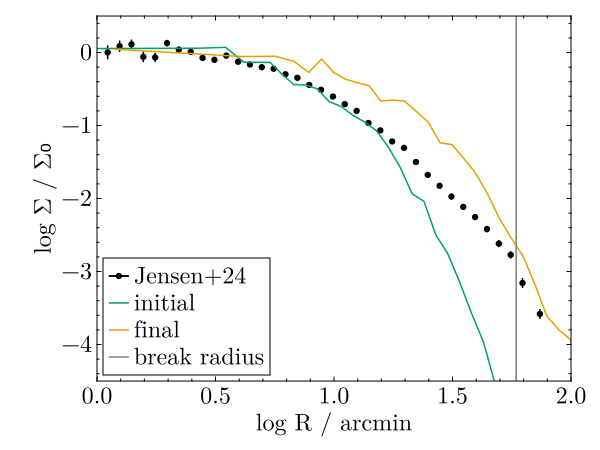
\includegraphics{figures/density_i_f.pdf}
    \caption{
        The stellar density of each model before (dotted) and after
        (solid) tidal evolution as compared to the observed density profile
        (solid points). The left and righ panels show results for Sculptor and
        Ursa Minor in the MW-only potential. The top and bottom panels show
        results for exponential and Plummer initial stellar conditions. We mark
        the half-light ($R_h$), the Jacobi radius, and break radius with arrows. 
}
    \label{fig:stellar_model_density}
\end{figure}


\begin{figure}
    \centering
    \includegraphics{figures/scl_lmc_density_i_f.pdf}
    \caption{
        Similar to Fig.~\ref{fig:stellar_model_density} except for Scl in the combined MW and LMC potential. The left and right panels show results for exponential and Plummer initial stellar profiles, respectively.
    }
    \label{fig:stellar_model_density_lmc}
\end{figure}

Fig.~\ref{fig:stellar_model_density} shows the initial and final stellar
densities of each galaxy in the MW-only potential compared to observations. The final profile resembles the initial profile
over the range of the observed density profile. UMi experiences the strongest evolution, with the stars expanding slightly and flattening past the break radius. But UMi's stars do not change measurably in shape. In addition, the break and Jacobi radii fall outside the observed stellar component, indicating that tidal effects should not be observable.

Since Scl and UMi may have been born with more extended stellar components, we
also consider Plummer initial stars, approximately matching the observed
density profiles. The Plummer profiles also remain nearly unchanged during
tidal evolution. If any tidal disturbances are visible, than observations would
have to probe more than two orders of magnitude fainter features than our data
reach. Therefore, tides do not substantively affect the observed stellar components of these models.

Fig.~\ref{fig:stellar_model_density_lmc} shows the tidal effects on Scl in the LMC+MW potential.
While the break radius coincides with the observed
excess, the Jacobi radius is too large to observe tidal signatures. In
addition, with a reduced number of pericentres compared to the MW-only case,
the stellar profiles evolve even less.

Not shown here, cored, anisotropic, and flattened models
all appear to evolve similarly over time. Given the observed velocity
dispersions, alternative dark matter structures still require a similar mass
within $R_h$ at the present day. Reasonable changes to the dark matter
structure likely do not change our conclusions.

A key caveat is that the long-term orbits of satellites are highly uncertain.
Analytic MW potentials neglect unknown details including triaxiality, mass
evolution, and substructure, causing analytic orbits to deviate significantly
from true satellite orbits \citep[e.g.,]{dsouza+bell2022, santistevan+2023}.
While we cannot constrain the long-term histories of these dwarfs, our results
indicate that {\it recent tidal effects} would not be observable in Scl and
UMi.

%%%%%%%%%%%%%%%%%%%%%%%%%%%%%%%%%%%%%%%%%%%%%%%%%%%%%%%%%%%%%%
\section{Discussion \& Conclusions}
We investigated whether tides from the Milky Way or LMC may explain the extended stellar densities of Scl and UMi. Using idealized N-body simulation on orbits with extreme pericentres, we find that tides are insufficient to influence the stellar light profile of either galaxy. We also find the LMC strongly perturbs Scl's orbit, weakining tides further. We conclude the observed density excess in Sculptor and Ursa Minor are unlikely to be tidal in origin.


Scl and UMi display other peculiarities that may hold clues to their formation. Both galaxies host at least two distinct chemodynamic populations
\citep{tolstoy+2004, battaglia+2008, pace+2020}.\footnotemark{} The inner population is
younger, higher metallicity, and dynamically colder, whereas the outer
population is older, lower metallicity, and dynamically hotter.
Fig.~\ref{fig:metallicity_gradient} compares a double-exponential density fit to the observed metallicity and velocity dispersion profiles. A double-exponential populations better explains the observed profiles than a single-exponential. Our two populations are similar to \citet[MMT]{pace+2020}. Though our second population is more extended than in \citet{arroyo-polonio+2024}, their third population may be contained within our outer component.

\footnotetext{Other examples of galaxies with multiple populations
  include Carina \citep{battaglia+2012, fabrizio+2016, kordopatis+2016},
  Fornax
  \citep{battaglia+2006, amorisco+evans2012, delpino+aparicio+hidalgo2015},
  Sextans
  \citep{battaglia+2011, cicuendez+battaglia2018, roederer+2023}, and
  Andromeda II
  \citep{mcconnachie+arimoto+irwin2007, ho+2012, delpino+2017}.}

\begin{figure}
    \includegraphics{figures/scl_umi_fe_h_gradient.pdf}

    \caption{
        {\bf Top:} Density profiles of Sculptor (top left) and Ursa Minor (top
        right) with double exponential fits (see
        appendix~\ref{sec:double_exp_fits}). Blue, pink, and red lines
        represent the inner, outer, and combined density, respectively.
        {\bf Middle:} The metallicities of member stars in both galaxies with
        radius. For Sculptor, we plot stars from
        APOGEE (green circles), \citet[][blue squares]{tolstoy+2023}, and
        \citet[][orange stars]{sestito+2023a}. For Ursa Minor, we
        plot stars from APOGEE (green circles), \citet[blue
        squares]{pace+2020}, and \citet[red stars]{sestito+2023b}. Black points
        represent median bins, and the pink line
        represent a simple mixture model of metallicity, transitioning from
        higher to lower metallicity based on the relative inner and outer
        component densities (see Table~\ref{tbl:double_exp_fits}). 
        {\bf Bottom:} The velocity dispersion profiles of our radial velocity
        sample (black points) as compared to the velocity dispersion profile
        for exponential profiles. We calculate the velocity dispersion of the
        model through the Jean's equations assuming a NFW dark halo of
        ($\rmax=2.5\,\kpc$, $\vmax=25\,\kms$) for Scl and ($\rmax=5\,\kpc$, $\vmax=27\,\kms$) for UMi.
    }
    \label{fig:metallicity_gradient}
\end{figure}

%Ursa Minor has also shown evidence for possible inner substructure, such
%as stellar or kinematic `clumps'
%\citep[e.g.,][]{olszewski+aaronson1985, demers+1995, kleyna+1998, battinelli+demers1999, bellazzini+2002}.
%While one clump was re-detected kinematically in \citet{pace+2014},
%\citet{munoz+2018} find no evidence of substructure with modern
%photometry. 
  We next consider a variety of possible origins.

\textbf{Episodic star formation.} Star formation may quench and
reignite, creating successive stellar generations with differing
distributions. External star formation triggers include tidal
compression \citep{mayer+2001a, dong+lin+murray2003}, collisions with
gaseous filaments or mergers \citep{genina+2019}, perturbations from dark halos
\citep{starkenburg+helmi+sales2016}, or shocks with the MW corona
\citep{wright+2019}.\footnote{More common mechanisms, like feedback or
reionization-driven quenching, may also form multiple stellar
generations
\citep{kawata+2006, benitez-llambay+2015, revaz+jablonka2018}. However,
such processes would not explain why extended stellar populations appear
to be non-universal.} In this case, the star formation history should
contain evidence of a corresponding burst.

\textbf{Major mergers.} In a dwarf merger, stars from
the lower-mass galaxy are preferentially dispersed, forming an extended
stellar component and population gradient
\citep{benitez-llambay+2016, deason+2022}. A halo may also form of many pre-reionization quenched ultra-faint dwarf galaxies \citep{ricotti+polisensky+cleland2022}. A few local dwarfs are
suspected to have undergone a major merger, including Tucana II,
Andromeda II, and Phoenix
\citep{lokas+2014, fouquet+2017, tarumi+yoshida+frebel2021, cardona-barrero+2021, querci+2025}.
A galaxy having undergone a major merger should harbour at least two or
three populations with distinct origin.

\textbf{Tidal preprocessing}. Some dwarf galaxies may have been tidally
`preprocessed' by a massive satellite like the LMC
\citep[e.g.,][]{santistevan+2023, riley+2024}. Tidal preprocessing
redistributes already-present stellar populations and may mimic a
stellar halo. Key evidence suggestive of preprocessing may include
distant dwarf stars or stellar streams.

\textbf{Dark-matter-free dwarfs.} Dark-matter-free tidal dwarfs 
%(formed in gas-rich tidal streams during the merger of two larger galaxies, e.g., \citealt{mirabel+dottori+lutz1992, bournaud+duc2006}) 
and galaxies in Modified Newtonian Dynamics (MOND) would be more susceptible to tides (\citealt{brada+milgrom2000, mcgaugh+wolf2010, casas+2012, yang+2014, wang+2024a}; but see also \citealt[][]{sanchez-salcedo+hernandez2007}).
In these cases, the high observed velocity dispersion requires evidence of strong tidal disruption, such as velocity gradients or tidal tails
\citep[e.g,][]{kroupa1997, read+2006, sanchez-salcedo+hernandez2007}. 

\textbf{Dynamical heating.} Old stars in dwarf galaxies may be
dynamically hotter than younger stars. Dynamical heating processes including
stellar feedback \citep{stinson+2009, maxwell+2012, el-badry+2016,
mercado+2021}, sub-subhalo interactions \citep{penarrubia+2025}, or even fuzzy
dark matter interference fringes \citep[e.g.,][]{el-zant+2020,
duttachowdhury+2023}. However, most of these processes should operate similarly
across dwarf galaxies, not just Scl and UMi.

While a number of scenarios may form an extended outer stellar density, future
observations have promise to discern different scenarios. 
{Precise chemistry}, comparing the inner and
outer regions, can test if the was accreted and could constrain properties
of merged satellites. 
{Detailed kinematics} could constrain the halo shape (ellipticity and anisotropy) and
if the dwarf shows signs of tidal disruption.
{Deep photometry} may find or rule out signs of dynamical
disequilibrium and tidal tails for tidally susceptible models and constrain the prevalence and nature of extended features in dwarf galaxies.
Finally, {star formation histories} may differentiate scenarios that rely on or create strong star formation bursts.
Both upcoming observatories and novel simulation methods will be instrumental to uncovering the formation histories of Sculptor and Ursa Minor.



%%%%%%%%%%%%%%%%%%%%%%%%%%%%%%%%%%%%%%%%%%%%%%%%%%%%%%%%%%%%%%
\begin{acknowledgements}
\end{acknowledgements}



\bibliographystyle{bibtex/aa.bst} % style aa.bst
\bibliography{paper.bib} % your references Yourfile.bib


\appendix


\section{Additional model results}
In this section, we present tables of the resulting properties of the dark matter and stellar components for each model. 

Tables~\ref{tbl:scl_orbit_props}, \ref{tbl:umi_orbit_props} contain information about the orbital properties of the models and our Monte carlo sampled orbits. Table~\ref{tbl:sim_results} contains the initial and final properties of the dark matter and stars for each simulation presented in the main text.



\begin{table}[t]
\centering
\caption[Observed Properties of Sculptor]{Observed properties of Sculptor. References are: (1) Muñoz et al. (2018, Sérsic fit), (2) Tran et al. (2022, RR lyrae distance), (3) Alan W. McConnachie and Venn (2020b), (4) Arroyo-Polonio et al. (2024). }
\label{tbl:scl_obs_props}
\begin{tabular}{lll}
\hline
parameter & value & Source\\
\hline
$\alpha / ^\circ$ & $15.0183 \pm 0.0012$ & 1\\
$\delta / ^\circ$ & $-33.7186 \pm 0.0007$ & 1\\
distance modulus & $19.60 \pm 0.05$ & 2\\
distance & $83.2 \pm 2$ kpc & 2\\
$\mu_{\alpha*} / \masyr$  & $0.099 \pm 0.002 \pm 0.017$ & 3\\
$\mu_\delta / \masyr$ & $-0.160 \pm 0.002_{\rm stat} \pm 0.017_{\rm sys}$  & 3\\
$\V_{\rm los}$ / ${\rm km\,s^{-1}}$ & $111.2 \pm 0.3\ $ & 4\\
$\sigma_v$ / ${\rm km\,s^{-1}}$ & $9.7\pm0.2\ $ & 4\\
$R_h/'$ & $9.79 \pm 0.04$ & 1\\
ellipticity & $0.37 \pm 0.01$ & 1\\
position angle & $94\pm1^\circ$ & 1\\
$M_V$ & $-10.82\pm0.14$ & 1\\
\hline
\end{tabular}
\end{table}

\begin{table}[t]
\centering
\caption[Observed Properties of Ursa Minor]{Observed properties of Ursa Minor. References are: (1) Muñoz et al. (2018, Sérsic fit), (2) Garofalo et al. (2025, RR lyrae distance), (3) Alan W. McConnachie and Venn (2020a), (4) Pace et al. (2020), average of MMT and Keck results with systematic uncertainty based on the difference between the MMT and Keck means. }
\label{tbl:umi_obs_props}
\begin{tabular}{lll}
\hline
parameter & value & Source\\
\hline
$\alpha/^\circ$ & $ 227.2420 \pm 0.0045$ & 1\\
$\delta/^\circ$ & $67.2221 \pm 0.0016$ & 1\\
distance modulus & $19.23 \pm 0.11$ & 2\\
distance/kpc & $70.1 \pm 3.6$ & 2\\
$\mu_\alpha*$ / mas yr$^{-1}$  & $-0.124 \pm 0.004 \pm 0.017$ & 3\\
$\mu_\delta$ / mas yr$^{-1}$  & $0.078 \pm 0.004_{\rm stat} \pm 0.017_{\rm sys}$ & 3\\
$\V_{\rm los}$ / km s$^{-1}$  &$-245.9 \pm 0.3_{\rm stat} \pm 1_{\rm sys}$ & 4\\
$\sigma_v$ & $8.6 \pm 0.3$ & 4\\
$R_h$ & $11.62 \pm 0.1$ & 1\\
ellipticity & $0.55 \pm 0.01$ & 1\\
position angle & $50 \pm 1^\circ$ & 1\\
$M_V$ & $-9.03 \pm 0.05$ & 1\\
\hline
\end{tabular}
\end{table}

\begin{table*}[t]
\centering
\caption{The orbital properties for Scl.}
\label{tbl:scl_orbit_props}
\begin{tabular}{llllllll}
\hline
Property & MW orbits & MW N-body & LMC orbits & LMC N-body \\
\hline
pericentre $/$ kpc & $53\pm3$ & 42 & $44 \pm 3$ & 39 \\
LMC pericentre $/$ kpc & -- & -- & $28.7^{+1.6}_{-1.6}$ & 20 \\
apocentre $/$ kpc & $102\pm3$ & 94 & $218 \pm 8$ & -- \\
time of last pericentre $/$ Gyr & $-0.45\pm0.2$ & $-0.47$ & $-0.38\pm0.01$ & $-0.33$ \\
time last peri LMC / Gyr & -- & -- & $-0.111\pm 0.003$ & -0.10 \\
number of pericentres & 5--6 & 6 & 1 & 1 \\
final heliocentric distance $/$ kpc & $83.2\pm2$ & 81.6 & --- & 72.9\\
\hline
Jacobi radius $/$ kpc & $4.5 \pm 0.3$ & 3.5 & $3.3\pm0.2$  & 2.8 \\
Jacobi radius $/$ arcmin & $186\pm12$ & 148 & $136 \pm 9$  & 132 \\
LMC Jacobi radius $/$ kpc & -- & -- &  $3.6\pm0.2$ & 2.6\\
LMC Jacobi radius $/$ arcmin & -- & -- &  $159\pm5$ & 121\\
\hline
break radius $/$ kpc & $-2.45\pm0.11$ & 2.6 & $-2.06\pm0.07$ & 1.82\\
break radius $/$ arcmin & $-101\pm4$ & 109 & $-85.1\pm2.1$ & 85 \\
LMC break radius $/$ kpc  & -- & -- & $-0.604^{+0.019}_{-0.019}$ & 0.56\\
LMC break radius $/$ arcmin & -- & -- & $-25\pm0.6$ & 27\\
\hline
\end{tabular}
\end{table*}


\begin{table*}[t]
\centering
\caption{Similar to Table~\ref{tbl:scl_orbit_props}, except for the orbital properties of UMi.}
\label{tbl:umi_orbit_props}
\begin{tabular}{llll}
\hline
Property &  MW orbits & MW N-body & LMC orbits\\
\hline
pericentre $/$ kpc & $37\pm3$ & 30 & $45.6^{+11.0}_{-8.2}$\\
LMC pericentre $/$ kpc & -- & -- & $118.1^{+3.7}_{-83.0}$ \\
apocentre $/$ kpc & $83\pm4$ & 75 &  $131.0^{+300.0}_{-18.0}$\\
time of last pericentre $/$ Gyr  & $-0.96\pm0.07$ & $-0.80$ & $-2.14^{+0.24}_{-0.29}$ \\
time of last peri LMC $/$ Gyr  & -- & -- & $-3.43^{+0.45}_{-0.71}$ \\
number of pericentres & 7--8 & 8 & $3\pm1$ \\
final heliocentric distance & $70.1\pm3.6$ & 64.7 & $70.1 \pm 3.6$\\
\hline
Jacobi radius $/$ kpc & $3.7\pm0.3$ & 2.9 & $5.2^{+1.3}_{-1.0}$ \\
Jacobi radius $/$ arcmin & $184\pm12$ & 156 & $259.0^{+54.0}_{-50.0}$ \\
LMC Jacobi radius $/$ kpc & -- & -- &  $22.2^{+0.71}_{-15.0}$ \\
LMC Jacobi radius $/$ arcmin & -- & -- & $1079.0^{+23.0}_{-730.0}$ \\
\hline
break radius $/$ kpc  & $-4.65^{+0.35}_{-0.39}$ & 3.9 &  $10.3^{+1.2}_{-1.5}$\\
break radius $/$ arcmin &  $-228.0^{+12.0}_{-13.0}$ & 206 & $507.0^{+45.0}_{-53.0}$ \\
LMC break radius $/$ kpc  & -- & -- & $16.6^{+2.3}_{-3.5}$ \\
LMC break radius $/$ arcmin & -- & -- &  $814.0^{+83.0}_{-130.0}$\\
\hline
\end{tabular}
\end{table*}


\begin{table}[t]
\centering
\caption{The simulation properties for Scl and UMi.}
\label{tbl:sim_results}
\begin{tabular}{llll}
\hline
Property & Scl MW & Scl LMC & UMi MW \\
\hline
$r_\textrm{max, f} / r_\textrm{max, i}$ & 0.406 & 0.763 & 0.249 \\
$\V_\textrm{max, f} / \V_\textrm{max, i}$ &  0.695 & 0.928 & 0.511 \\
$f_{\rm lost, DM}$ & 0.917 & 0.451 & 0.965 \\
\hline
$R_{h, \rm exp, i} / \kpc$ &  0.168 & 0.186 & 0.168\\
$R_{h, \rm exp, f}/\kpc$ &  0.189 & 0.189 & 0.212\\
$\sigma_{h, \rm exp, i}/\kms$ & 9.8 & 9.0 & 11.0 \\
$\sigma_{h, \rm exp, f}/\kms$ & 8.8 & 8.8 & 8.8 \\
$f_{\rm lost, exp}$ & $2.1\times 10^{-6}$ & $5\times10^{-13}$ & 0.0014\\
\hline
$R_{h, \rm Plummer, i}/\kpc$ & 0.202 & 0.201 & 0.201 \\
$R_{h, \rm Plummer, f}/\kpc$ & 0.227 & 0.205 & 0.257\\
$\sigma_{h, \rm Plummer, i}/\kms$ & 10.7 & 9.4 & 12.1\\
$\sigma_{h, \rm Plummer, f}/\kms$ & 9.4 & 9.2 & 9.1\\
$f_{\rm lost, Plummer}$ & $0.024$ & 0.0013 & 0.068\\
\hline
\end{tabular}
\end{table}

% Fig.~\ref{fig:umi_sim_images} shows the dark matter evolution of our UMi
% model, the most tidally affected model. The dark matter creates large wakes and
% streams encircling the Galaxy several times, but the inner dark matter
% structure remains intact (not shown).


%\begin{figure}
%    \centering
%    \includegraphics[width=\columnwidth]{figures/umi_sim_images.png}
%    \caption{
%        Images of Ursa Minor's dark matter over a selection of past apocentres
%        and the present day. The colours represent the projected DM density in
%        the $y$-$z$ plane, scaled to be logarithmic over 5 orders of magnitude.
%        The green dot represents the final expected position of the galaxy, and
%        the solid and dotted grey curves represent the orbit over one previous
%        or future radial oscillation, respectively.
%}
%    \label{fig:umi_sim_images}
%\end{figure}


\section{Fits to density profiles and metallicity gradients}

\subsection{Spectroscopic sample selection} \label{sec:velocity_sample}
To create a sample of spectroscopic members, we compile LOS velocities from
several surveys. For
Sculptor, we combine \citet{tolstoy+2023}; \citet{walker+2009};
\citet{sestito+2023a}; and APOGEE \citep[DR17,][]{abdurrouf+2022}. For
Ursa Minor, we combine \citet{spencer+2018}; \citet{pace+2020};
\citet{sestito+2023b}; and APOGEE. We then cross-match all catalogues to
J+24 Gaia stars. If a study did not report \emph{Gaia} DR3 source IDs,
we match to the nearest star within 1--3 arcseconds. We combine
measurements of the same star using inverse-variance weighting. To
reduce likely binaries, we remove stars with significant velocity
dispersions.\footnote{Specifically, using that
  \(\chi^2=\frac{s^2}{\delta \bar v^2}\), we remove stars with a
  \(\chi^2\) larger than the 99.9th percentile of the \(\chi^2\)
  distribution with \(N-1\) measurements.}

We build on J+24's likelihood by adding multiplicative terms in the
total likelihood for the velocity consistency. We assume that the satellite and
background \(v_{\rm los, gsr}\) distributions are Gaussian in the
Galactic Standard of Rest (GSR, i.e., same location as ICRS but
velocities relative to the galactic centre). For the satellite, we adopt
a mean and standard deviation based on
Tables~\ref{tbl:scl_obs_props}, \ref{tbl:umi_obs_props}, and, for the
background, mean \(0\,\kms\) and dispersion
\(\sigma_{\rm halo} = 100\,\kms\) \citep[e.g.][]{brown+2010}. We select
stars with velocity-informed satellite membership probabilities of
greater than 0.2. For Scl, we find 1918 unique members and UMi, 831.

For UMi, we shifted the velocities of \citet{spencer+2018}
(\(-1.1\,\kms\)) and \citet{pace+2020} (\(+1.1\,\kms\) ) to account for
a systematic velocity offset. Otherwise, all studies appear to be on a
similar velocity scale.

We correct the velocities for the solar motion and the on-sky size of
the galaxy. We transform the velocities into the GSR and correct for the
apparent gradient induced by the dwarf's proper motion
\citep[see,][]{WMO2008, strigari2010}. The
correction from both effects induces an apparent gradient of about
$1.3\,{\rm km\,s^{-1}\,deg^{-1}}$ for Sculptor and less for Ursa Minor. 

\subsection{Density profile fits} \label{sec:double_exp_fits}

Here, we describe our fitting procedure to derive the double exponential fits and metallicity gradients in Fig.~\ref{fig:metallicity_gradient}.

For the double exponential fits, we extend \citet{jensen+2024} to fit a double exponential with free inner and outer parameters. Specifically, we use a similar likelihood formulation except we hold the proper motion likelihood fixed, and allow the inner and outer density components to include free position angle, ellipticity, scale radius, and fit for the relative total mass of the outer component $f_{\rm outer}$. We perform the fits using the No-U Turn Sampler (an adaptive Hamilton-Monte Carlo algorithm), assuming uniform priors for position angle and ellipticity, and log-uniform priors for scale radius.

To fit the metallicity gradient, we instead assume that the density profile follows the double exponential fit above, and then fit a mixture model of the metallicity gradient as a sum of two Gaussian distributions. The four free parameters of this model are the mean and metallicity dispersion of the inner and outer components. 

Table~\ref{tbl:double_exp_fits} contain the derived parameters and quantile uncertainties for both Scl and UMi. We find strong evidence for multiple populations with different mean metallicities. Our outer population scale radius is smaller than in \citet{jensen+2024} for Scl but is similar for Ursa Minor. 


\begin{table}
\centering
\caption{The double exponential fit results for Scl and UMi}
\label{tbl:double_exp_fits}
\begin{tabular}{lllll}
\hline
Parameter & Scl  & Scl  & UMi  & UMi  \\
 & inner & outer & inner & outer \\
\hline
$R_h$ & $7.85^{+0.32}_{-0.33}$ & $17.1^{+1.3}_{-1.2}$ & $10.58^{+0.52}_{-0.42}$ & $29.7^{+3.4}_{-3.2}$\\
$\theta$ & $98.8^{+4.2}_{-4.0}$ & $91.8^{+3.0}_{-3.1}$ & $50.4^{+1.7}_{-1.6}$ & $74.0^{+68.0}_{-45.0}$ \\
ell & $0.243^{+0.031}_{-0.034}$ & $0.383^{+0.035}_{-0.036}$ & $0.598^{+0.025}_{-0.029}$ &  $0.087^{+0.086}_{-0.059}$ \\
$f_{\rm outer}$ & --- & $0.315^{+0.058}_{-0.052}$ & --- & $0.249^{+0.043}_{-0.041}$ \\
\hline
$\mu_{\rm [Fe/H]}$ &  $-1.671^{+0.021}_{-0.021}$ &  $-1.982^{+0.024}_{-0.024}$ & $-2.147^{+0.02}_{-0.02}$ & $-2.523^{+0.095}_{-0.087}$ \\
$\sigma_{\rm [Fe/H]}$ & $0.574^{+0.016}_{-0.015}$ & $0.336^{+0.019}_{-0.018}$ & $0.347^{+0.015}_{-0.014}$ & $0.505^{+0.067}_{-0.066}$ \\
\hline
\end{tabular}
\end{table}



\end{document}
